\newpage

\section{Landmarks} \label{section:landmarks}

Są to punkty nakładane na twarz wokół interesujących obszarów - takich jak oczy, nos czy usta. Pozwalają określić położenie, rozmiar czy kształt tych obiektów. Mogą być również użyte do predykcji czy mamy zamknięte/otwarte oczy lub czy się uśmiechamy. 

\subsection{OpenCV-contrib}
Dodatkowe moduł opencv facemark (\textit{OpenCV-contrib}) zawiera trzy algorytmy detekcji landmarków:

\begin{itemize}
    \item Kazemi
    \item AAM
    \item LBF
\end{itemize}

\subsubsection{FacemarkLBF}

Używając metody FacemarkLBF oraz modelu \textit{lbfmodel.yaml} określiłem punkty orientacyjne twarzy. \cite{landmarkSatyaMallick}

\begin{figure}[!h]
    \begin{center}
        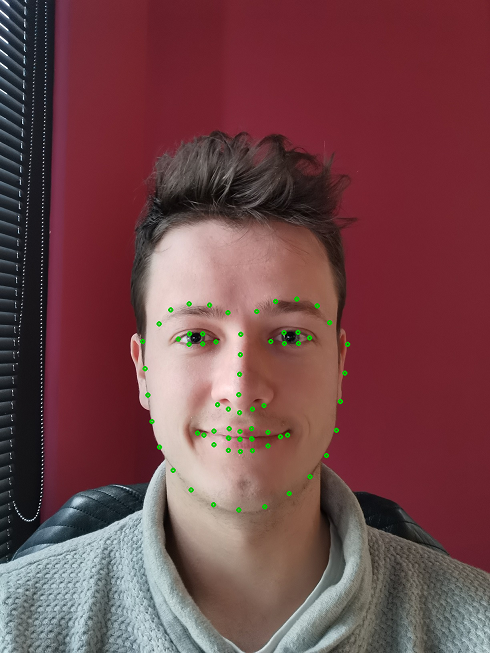
\includegraphics[scale=0.6]{img/landmark_section/landmarks_1.png}
        \caption{Twarz z naniesionymi landmarkami}
        \label{fig:landmarks_1}
    \end{center}
\end{figure}

